%!TEX root = /Users/kevin/SkyDrive/KTH Work/Period 3 2014/DN2255/Homework/1/Heat Equation/Heat Equation.tex
\section{Discretization and implementation} 

% (fold)
\label{sec:discretization_and_implementation} 
\begin{figure}[htbp] 
	\centering 
	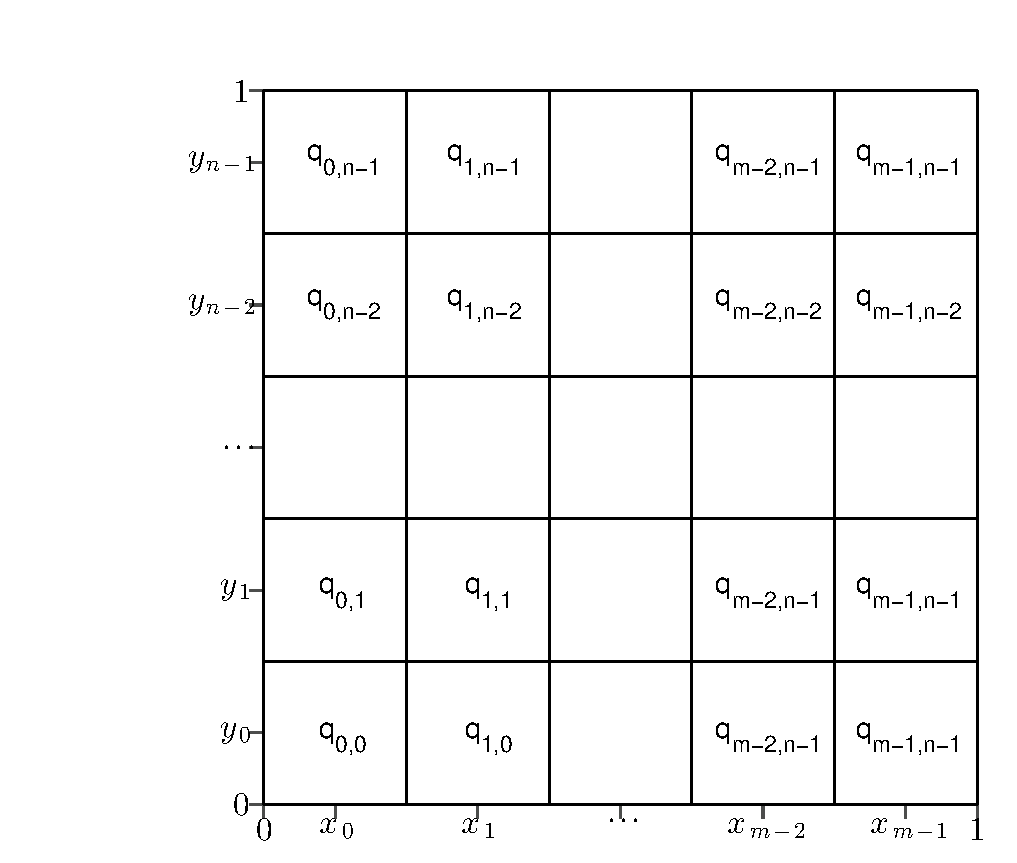
\includegraphics[width=.7\textwidth]{Figures/gridForNumericalSchemePlot.eps} \caption{Finite volume grid} \label{fig:Figures_gridForNumericalSchemePlot} 
\end{figure}

Let $Q_{ij}$ denote the cell average of q over cell (i,j) so, 
\begin{equation}
	Q_{ij}(t) = \frac{1}{\Delta x \Delta y} \int_{x_{i-1/2}}^{x_{i+1/2}}\int_{y_{j-1/2}}^{y_{j+1/2}} q(x_i,y_j,t) dxdy \label{eq:qCellAverage} 
\end{equation}
and defining $S_{ij}$ as the cell average of S over cell (i,j), 
\begin{equation}
	S_{ij}(t) = \frac{1}{\Delta x \Delta y} \int_{x_{i-1/2}}^{x_{i+1/2}}\int_{y_{j-1/2}}^{y_{j+1/2}} S(x_i,y_j,t) dxdy \label{eq:sCellAverage} 
\end{equation}
where $\Delta x = x_{i+1/2}-x_{i-1/2}$ and $\Delta y = y_{j+1/2}-y_{j-1/2}$ 
\begin{enumerate}
	\item Derive a finite volume method for the spatial part of (\ref{eq:equation1}) by integrating and forming cell averages. 
	\begin{align*}
		& q_t = \nabla \cdot (\nabla q) + S \\
		& \iint \limits_{\Delta x \, \Delta y} q_t = \iint \limits_{\Delta x \, \Delta y} \nabla^2 q + \iint \limits_{\Delta x \, \Delta y} S \\
		& \frac{d}{dt} \iint \limits_{\Delta x \, \Delta y} q = \iint \limits_{\Delta x \, \Delta y} \left( \frac{d^2 q}{dx^2} + \frac{d^2 q}{dy^2} \right) + \iint \limits_{\Delta x \, \Delta y} S 
	\end{align*}
	and now dividing everything by the common cell area $\Delta x \Delta y$, we can use (\ref{eq:qCellAverage}) and (\ref{eq:sCellAverage}) to get 
	\begin{align}
		& \frac{d}{dt} Q_{ij}(t) = \frac{1}{\Delta x \Delta y}\iint \limits_{\Delta x \, \Delta y} \left( \frac{d^2 q}{dx^2} + \frac{d^2 q}{dy^2} \right) + S_{ij}(t) \label{eq:eqCommon} 
	\end{align}
	
	I will Taylor expansions to define the Laplacian terms. The Taylor expansions of $q(x_i+\Delta x)$ and $q(x_i-\Delta x)$, taking the derivative with respect to x are
	
	% \begin{align*}
	% 	& q(x_i+\Delta x) = q(x_i) + \Delta x \, q'(x_i) + \frac{1}{2} (\Delta x)^2 q''(x_i) + \frac{1}{6} (\Delta x)^3 q'''(\zeta_+) \\
	% 	& q(x_i-\Delta x) = q(x_i) - \Delta x \, q'(x_i) + \frac{1}{2} (\Delta x)^2 q''(x_i) - \frac{1}{6} (\Delta x)^3 q'''(\zeta_-) 
	% \end{align*}
	\begin{align}
		& q(x_i+\Delta x) = q(x_i) + \Delta x \, q'(x_i) + \frac{1}{2} (\Delta x)^2 q''(x_i) + \frac{1}{6} (\Delta x)^3 q'''(x_i) + \frac{1}{24} (\Delta x)^4 q^{(4)}(\zeta_+) \label{eq:taylorExp1}\\
		& q(x_i-\Delta x) = q(x_i) - \Delta x \, q'(x_i) + \frac{1}{2} (\Delta x)^2 q''(x_i) - \frac{1}{6} (\Delta x)^3 q'''(x_i) + \frac{1}{24} (\Delta x)^4 q^{(4)}(\zeta_-) \label{eq:taylorExp2} 
	\end{align}
	where the last terms represent a value $\zeta_\pm$ that makes the truncation of the Taylor expansion exactly equal to the infinite series. Since we do not know this value, we must remove it and it will be our truncation error. Adding (\ref{eq:taylorExp1}) with (\ref{eq:taylorExp2}) and rearranging terms, 
	\begin{align*}
		& q''(x_i) = \frac{q(x_i + \Delta x) + q(x_i-\Delta x) - 2 q(x_i)}{(\Delta x)^2} - \frac{1}{12} (\Delta x)^2 q^{(4)}(\zeta) 
	\end{align*}
	and taking off the truncation error, 
	\begin{align*}
		& q''(x_i) = \frac{q(x_i + \Delta x) + q(x_i-\Delta x) - 2 q(x_i)}{(\Delta x)^2} 
	\end{align*}
	Doing the same thing for $y_j$ and $\Delta y$ 
	\begin{align*}
		& q''(y_j) = \frac{q(y_j + \Delta y) + q(y_j-\Delta y) - 2 q(y_j)}{(\Delta y)^2} 
	\end{align*}
	Now substituting these equations back into (\ref{eq:eqCommon}), rewriting $q(x_i\pm\Delta x)$ as $q_{i\pm1,j}$, $q(y_j\pm\Delta y)$ as $q_{i,j\pm1}$, and for this problem,$\Delta x = \Delta y$,
	
	% \begin{align}
	% 	& \frac{d}{dt} Q_{ij}(t) = \iint \limits_{\Delta x \, \Delta y} \left( \frac{ q_{i+1,j} +q_{i-1,j}-2q_{i,j}}{(\Delta x)^2} + \frac{q_{i,j+1} + q_{i,j-1} -2q_{i,j} }{(\Delta y)^2} \right) + S_{ij}(t)
	% \end{align}
	\begin{align}
		& \frac{d}{dt} Q_{ij}(t) = \frac{1}{\Delta x \Delta y} \iint \limits_{\Delta x \, \Delta y} \left( \frac{ q_{i+1,j} +q_{i-1,j} +q_{i,j+1} + q_{i,j-1} -4q_{i,j} }{\Delta x \Delta y} \right) + S_{ij}(t) \label{eq:dLaplacian} 
	\end{align}
	Lastly, it can be seen that (\ref{eq:dLaplacian}) is the 5-point Laplacian combined with the average of q over a cell which is $Q_{ij}$, so the equation becomes 
	\begin{align*}
		& \frac{d}{dt} Q_{ij}(t) = \left( \frac{ Q_{i+1,j} +Q_{i-1,j} +Q_{i,j+1} + Q_{i,j-1} -4Q_{i,j} }{\Delta x \Delta y} \right) + S_{ij}(t) \\
		& \frac{d}{dt} Q_{ij}(t) = \Delta_5 Q_{ij} + S_{ij}(t) 
	\end{align*}
	\\
	At the boundaries, there is no flux, F=0, so $Q_{0,j}=Q_{-1,j}$, $Q_{i,0}=Q_{i,-1}$, $Q_{i,N-1}=Q_{i,N}$, $Q_{M-1,j}=Q_{M,j}$. The stencils for corner boundaries like $i=0,j=0$ or $i=m-1,j=n-1$
	
	% \begin{equation*}
	% 	\frac{d}{dt} Q_{ij}(t) = \left( \frac{ Q_{i+1,j} +Q_{i-1,j} +Q_{i,j+1} + Q_{i,j-1} -4Q_{i,j} }{\Delta x \Delta y} \right) + S_{ij}(t) 
	% \end{equation*}
	\begin{align}
		\frac{d}{dt} Q_{0,0}^n &= \left( \frac{ Q_{1,0} +Q_{-1,0} +Q_{0,1} + Q_{0,-1} -4Q_{0,0} }{\Delta x \Delta y} \right) + S_{0,0}(t) \\
		&= \left( \frac{ Q_{1,0} +Q_{0,1} -2Q_{0,0} }{\Delta x \Delta y} \right) + S_{0,0}(t) \\
		\frac{d}{dt} Q_{m-1,j-1}^n &= \left( \frac{ Q_{m-2,j-1} +Q_{m-1,j-2} -2Q_{m-1,j-1} }{\Delta x \Delta y} \right) + S_{m-1,j-1}(t) 
	\end{align}
	Equations for boundaries not at a corner look like this: 
	\begin{align}
		\begin{cases}
			\frac{d}{dt} Q_{i,0}^n = \left( \frac{ Q_{i+1,0} +Q_{i-1,0} +Q_{i,1} + -3Q_{i,0} }{\Delta x \Delta y} \right) + S_{i,0}, &\text{ if }i \neq 0,m-1 \text{ and }j=0 \\
			\frac{d}{dt} Q_{i,0}^n = \left( \frac{ Q_{i+1,0} +Q_{i-1,0} +Q_{i,1} + -3Q_{i,0} }{\Delta x \Delta y} \right) + S_{i,0}, &\text{ if } i \neq 0,m-1 \text{ and }j=N-1 \\\\
			\frac{d}{dt} Q_{0,j}^n = \left( \frac{ Q_{1,j} +Q_{0,j+1} + Q_{0,j-1} -3Q_{0,j} }{\Delta x \Delta y} \right) + S_{0,j},  &\text{ if }i = 0 \text{ and }j\neq 0,N-1 \\\\
			\frac{d}{dt} Q_{m-1,j}^n = \left( \frac{Q_{m-2,j} +Q_{m-1,j+1} + Q_{m-1,j-1} -3Q_{m-1,j} }{\Delta x \Delta y} \right) + S_{m-1,j},  &\text{ if }i = m-1 \text{ and }j\neq 0,N-1 \\
		\end{cases}
	\end{align}
	\item Integrate with implicit Euler scheme 
	\begin{align}
		& \frac{Q_{ij}^{n+1}-Q_{ij}^{n}}{\tau} = \Delta_5 Q_{ij}^{n+1} + S_{ij}^n(t) \\
		& Q_{ij}^{n+1} = (\mathbf{I}-\tau \mathbf{\Delta_5})^{-1} (Q^n+S^n) 
	\end{align}
	
	The implicit Euler scheme is unconditionally stable where the explicit scheme has restrictions on the time step.  To find the stability of $\mathbf{Q}^{n+1}=\mathbf{A}\mathbf{Q}^n$, we find the eigenvalues of $\mathbf{A} v_k=\lambda_k v_k$.  The temperature at a later time can be written in terms of the initial temperature by multiplying the matrix $\mathbf{A}$ by itself $n$ times, $\mathbf{Q}^{n+1}=\mathbf{A}^n\mathbf{Q}^1$. If any eigenvalue of $\mathbf{A}$ satisfies $|\lambda_k|>1$, then as $n \to \infty$, $Q \to \infty$.\cite{garcia2000numerical}
	The explicit scheme has a value where the eigenvalue could become greater than one.  But the implicit scheme takes the inverse of a matrix before the eigenvalues are calculated, thus making the maximum absolute value of an eigenvalue never greater than zero.
	\item The laplacian written as the second derivative in 1D for each dimension is convenient because this allows us to easily define the boundary conditions similar to like we would for a purely 1D system.  
	\begin{itemize}
		\item[i.]  The fully discrete problem in matrix form
		\begin{align*}
			& Q_{ij}^{n+1}(t) = (\mathbf{I}-\tau (\mathbf{T_x} + \mathbf{T_y}))^{-1} (Q^n+S^n) 
		\end{align*}
		where $\mathbf{T_{x}} = \frac{1}{\Delta x^2}(\delta_{i-1} + \delta_{i+1} - 2\delta_{i})$ and $\mathbf{T_{y}} = \frac{1}{\Delta y^2}(\delta_{j-1} + \delta_{j+1} - 2\delta_{j})$.  
		
		Near an x or y boundary, one term from that respective derivative will cancel with the $2 \delta_i,j$ term.  For example, when $i=0$, $\mathbf{T_{x}}$ will become $\frac{1}{\Delta x^2}( \delta_{i+1} - \delta_{i})$ because the $\delta_{i-1}$ term will cancel with a $\delta_{i}$ term because of boundary conditions.
	\end{itemize}
	
	\item {\color{blue} The method was implemented using the operator matrix $\mathbf{A}$ \cite{Demmel:1997:ANL:264989} and is generated at line 1 in the code.  The sparse function was also used on the matrix to save computational power and time
	\begin{equation}
			A = \left[
			\begin{tabular}{ccc|ccc|ccc}
			4  & -1 & 0		& -1 & 0 & 0 	& 0 & 0 & 0\\
			-1 & 4  & -1 	& 0 & -1 & 0 	& 0 & 0 & 0\\
			0  & -1 & 4  	& 0 & 0 & -1 	& 0 & 0 & 0\\
			\midrule
			-1 & 0  & 0  	& 4 & -1 & 0 	& -1 & 0 & 0\\
			0  & -1 & 0  	& -1 & 4 & -1 	& 0 & -1 & 0\\
			0  & 0  & -1 	& 0 & -1 & 4 	& 0 & 0 & -1\\
			\midrule
			0  & 0  & 0  	& -1 & 0 & 0 	& 4 & -1 & 0\\
			0  & 0  & 0  	& 0 & -1 & 0 	& -1 & 4 & -1\\
			0  & 0  & 0  	& 0 & 0 & -1 	& 0 & -1 & 4\\
			\end{tabular}\right]
			\label{eq:matrixA}
		\end{equation}}
\end{enumerate}

% section discretization_and_implementation (end)
